%\documentclass[12pt,english]{article}
%\usepackage{fullpage}
%\usepackage[T1]{fontenc} 
%\usepackage{helvet}
%\renewcommand{\familydefault}{\sfdefault}
%\usepackage{babel}
%\usepackage{amsmath}
%\numberwithin{equation}{section}
%\usepackage{hyperref}
%\usepackage{tikz,pgfplots}
%\usepackage{boldline} %To get thicker lines in tables
%\usepackage{float}    %For float on figures for exampel
%\usepackage{graphicx} %Figures
%
%\usepackage{sectsty}
%\allsectionsfont{\centering}
%
%\renewcommand{\thesubsection}{\Roman{subsection}} 
%\renewcommand{\thesubsubsection}{\Alph{subsubsection}} 
%
%\newcommand{\ignore}[1]{}
%
%\begin{document}
%
%\begin{figure}[H]
%  \centering
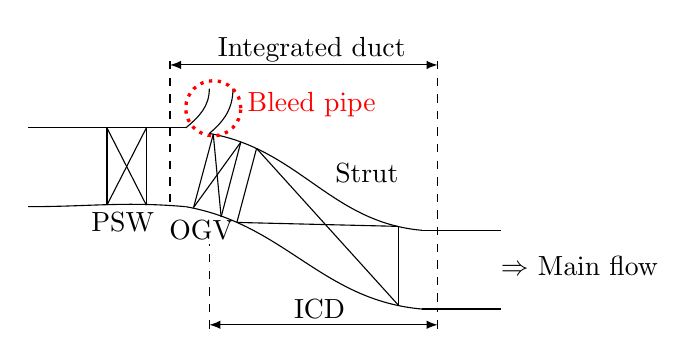
\begin{tikzpicture}
  \coordinate (A) at (-1,1);
  \coordinate (B) at (1,1);
  \coordinate (C) at (1.3,1.5);
  \coordinate (D) at (1.6,1.5);
  \coordinate (E) at (1.3,0.93);
  \coordinate (F) at (4,-0.3);
  \coordinate (G) at (5,-0.3);
  \coordinate (H) at (-1,0);
  \coordinate (I) at (1,0);
  \coordinate (J) at (4,-1.3);
  \coordinate (K) at (5,-1.3);
  %Upper side
  \draw (A)--(B);
  \path [black,out=40,in=-90] (B) edge (C);
  \path [black,out=-90,in=40] (D) edge (E);
  \path [black,out=-10,in=175] (E) edge (F);
  \draw (F)--(G);
  \draw[red,dotted, very thick] (1.35,1.25) circle (0.35);
  \node[red] at ([shift={(1.0,-0.2)}]D) {Bleed pipe};
  %Lower side
  \path [black,out=0,in=175] (H) edge (I);
  \path [black,out=-10,in=175] (I) edge (J);
  \path [black,out=0,in=180] (J) edge (K);
  %PSW
  \draw (0,1)--(0,0.02);
  \draw (0.5,1)--(0.5,0.02);
  \draw (0,0.02)--(0.5,1.0);
  \draw (0.5,0.02) -- (0,1);
  %\node at ([shift={(1.2,0.2)}]A) {PSW};
  %OGV
  \draw (1.35,0.92) -- (1.1,-0.01);
  \draw (1.7,0.82) -- (1.45,-0.13);
  \draw (1.35,0.92) -- (1.45,-0.13);
  \draw (1.7,0.82) -- (1.1,-0.01);
  %\node at ([shift={(0.0,-0.3)}]I) {OGV};
  %Duct
  \draw (1.9,0.74) -- (1.65,-0.2);
  \draw (3.7,-0.25) -- (3.7,-1.25);
  \draw (1.9,0.74) -- (3.7,-1.25);
  \draw (3.7,-0.25) -- (1.65,-0.2);
  %\node at ([shift={(1.8,-0.5)}]E) {Duct};

  %Marking the Integrated duct
  \node at ([shift={(1.0,0.5)}]D) {Integrated duct};
  \draw[latex-latex] (0.8,1.8)--(4.2,1.8);
  \draw[dashed] (0.8,1.85)--(0.8,0);
  \draw[dashed] (4.2,1.85)--(4.2,-1.3);
  %Marking the duct
  \node at ([shift={(-1.3,0.)}]J) {ICD};
  \draw[latex-latex] (1.3,-1.5)--(4.2,-1.5);
  \draw[dashed] (1.3,-1.55)--(1.3,-0.48);
  \draw[dashed] (4.2,-1.55)--(4.2,-1.3);

  %Mark Front Traverse surface
  %\draw[dashed, thick] (0.8,1.2)--(0.8,0);
  %Strut
  \node at ([shift={(2.0,-0.5)}]E) {Strut};
  %PSW
  \node at ([shift={(1.2,-0.2)}]H) {PSW};
  %OGV
  \node at ([shift={(0.2,-0.3)}]I) {OGV};
  %Main flow
  \node at ([shift={(1.0,-0.45)}]G) {$\Rightarrow$ Main flow};
\end{tikzpicture}
%  \caption{Schematic of the integrated compressor duct design}
%  \label{fig:schema}
%\end{figure}
%\end{document}
